\chapter{Pontos de Interesse}\label{sec:pontosdeinteresse}
%======================================================================================
%
A reconstrução 3D pelo método da estrutura do movimento, ou {\it Structure from Motion} (\it{SfM}). Tem como base a utilização de pontos de interesse
(\it features), que são pontos ou áreas em comum entre as imagens usadas na reconstrução. Para encontrar estes pontos, diferentes algoritmos são empregados.

\section {{\it SIFT - Scale Invariant Feature Transform}}

Primeiramente, utiliza-se o SIFT (algoritmo de detecção de pontos de interesse, invariante à escala e à transformações, como rotação, translação e iluminação da imagem, por exemplo).
O algoritmo pode ser dividido em cinco etapas, das quais:

\begin{itemize}
	\item{Deteccão de espaço de escala Extrema - {\it Scale-space Extrema Detection}}
	\item{Localização de pontos chaves - {\it Keypoint Localization}}
	\item{Atribuição de orientação - {\it Orientation Assignment}}
	\item{Descritor de pontos chaves - {\it Keypoint Descriptor}}
	\item{Combinação de pontos chaves - {\it Keypoint Matching}}
\end{itemize}


\subsection{Deteccão de espaço de escala Extrema}

% From the image above, it is obvious that we can't use the same window to detect keypoints with different scale. It is OK with small corner. But to detect larger corners we need larger windows. For this, scale-space filtering is used. In it, Laplacian of Gaussian is found for the image with various σ values. LoG acts as a blob detector which detects blobs in various sizes due to change in σ. In short, σ acts as a scaling parameter. For eg, in the above image, gaussian kernel with low σ gives high value for small corner while guassian kernel with high σ fits well for larger corner. So, we can find the local maxima across the scale and space which gives us a list of (x,y,σ) values which means there is a potential keypoint at (x,y) at σ scale.

Em casos com cantos pequenos, a detecção funciona bem. Porém, raramente utilizaremos a mesma janela para detectar pontos chaves em imagens com diferentes escalas, pois utilizamos imagens grandes e, consequentemente, cantos grandes. Para isso, precisamos de janelas grandes também. Para resolver este problema, o filtro de escala-espaço é usado: o Laplaciano de Gaussiano (Laplacian of Gaussian "{\it LoG}"). O LoG atua como um detector de particulas em diferentes tamanhos $\sigma$. (Onde $\sigma$ é o parâmetro de escala). Por exemplo, o {\it kernel} gaussiano com $\sigma$ baixo, tem como resposta um alto valor para um canto pequeno. Enquanto um {\it kernel} gaussiano com alto $\sigma$, se encaixa bem para um canto maior. Com esta lógica, podemos encontrar um máximo local através da escala e o espaço, o que nos fornece uma lista de $(x,y \sigma)$, o que significa que existe um ponto chave em potencial, com o par $(x,y)$ na escala $\sigma$.

% \begin{equation}
% LoG(x,y) = - \frac{1}{\pi \sigma ^4 }\left [ 1 - \frac{x^2+y^2}{2 \sigma ^2} \right ]e^{- \frac{x^2+y^2}{2 \sigma ^2}} 
% \end{equation}

Porém, como o LoG é um pouco custoso, computacionalmente. O SIFT utiliza um algoritmo aproximado do LoG, o DoG (Diferença de Gaussianos - {\it Difference of Gaussians}). O DoG é a diferença de um filtro Gaussiano de uma imagem, com dois valores diferentes de escala $\sigma$. 
Uma aplicação prática do filtro DoG é a sequência de imagens a seguir:

\begin{figure} [!h]
	\centering
	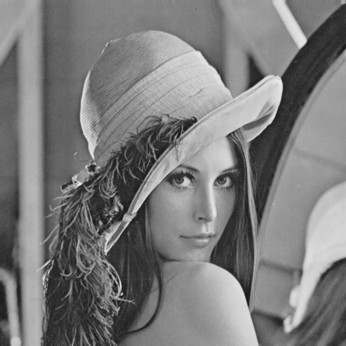
\includegraphics[width=0.45\linewidth]{figs/lena.jpg}(a)
	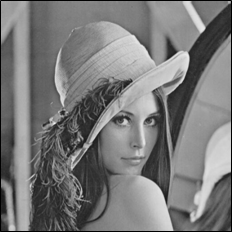
\includegraphics[width=0.45\linewidth]{figs/lenaSigma1.png}(b)
	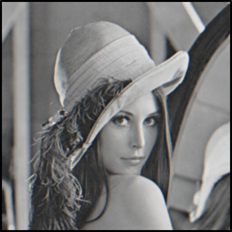
\includegraphics[width=0.45\linewidth]{figs/lenaSigma2.png}(c)
 	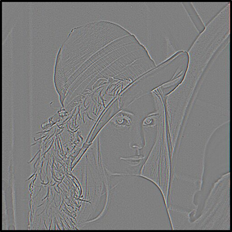
\includegraphics[width=0.45\linewidth]{figs/lenaDoG.png} (d)
	\caption{%
	É aplicado um filtro gaussiano na imagem original (a), com $\sigma$ = 1, tendo como resultado a imagem (b).
	Um outro filtro gaussiano é usado, porém, neste caso, o $\sigma$ = 2 (c). Após isso, subtrai-se (b) de (c), obtendo 
	o filtro DoG (d).
	}\label{fig:lenadog}
\end{figure}



No caso, as funções ficariam da seguinte forma: 

\begin{equation}
	h_\sigma(u,v) = \frac{1}{2 \pi \sigma ^2} e^{-\frac{u^2+u^2}{2 \sigma ^2}}
	\label{eq:gaussiano}
\end{equation}

\begin{equation}
\triangledown^2	h_\sigma(u,v)
	\label{eq:LoG}
\end{equation}

\begin{equation}
	\frac{\partial}{\partial x}h_\sigma(u,v)
	\label{eq:DoG}
\end{equation}


Onde \ref{eq:gaussiano} é a função padrão do operador gaussiano, a equação \ref{eq:LoG} é o operador LoG,  \ref{eq:DoG} é o operador DoG e $\triangledown^2$ é o operador Laplaciano.

%No presente trabalho, nos concentramos na configuração do tanque de onda
%oceânica descrita na Seção~\ref{sec:setup}, composta por quatro vídeos
%\emph{Full HD} tirados de diferentes pontos de vista em widebaseline. Cada vídeo tem cerca de 300 MB de
%resolução 1920x1080 e 30 fps.
%
%\section {Arquitetura de Implementação}
%
%Nosso sistema prático foi projetado para C++ usando as bibliotecas de visão 
%computacional VXL e VXD~\cite{vxl,vxd}. A linguagem C++ é rápida e escalável, e muitas
%vezes é a única solução para as grandes quantidades de processamento de vídeo que
%visamos. Além disto, escolhemos utilizar uma solução baseada em VXL por ser
%amplamenta utilizada na indústria, pela sua suite de testes e, também, por
%prover a opção de utilizar OpenCV caso necessário. A VXL é internamente utilizada
%por empresas como a General Electrics, a Vision Systems Inc, a Google, e uma
%série de startups e universidades, para sistemas de visão maiores e mais
%experimentais do que o OpenCV.
%
%Na prática, no entanto, foram apenas implementados os filtros treinados finais e
%os sinais (\emph{features}) em C++, com base no código Matlab de referência
%por~\etal~\cite{Guo:etal:CVPR14,Guo:etal:PAMI2017:submitted}. Nosso código 
%C++ é aberto na biblioteca VXD e já foi usado pela
%Brown University e outros pacotes~\cite{Yuliang:edge:detection:github}. Decidimos 
%manter o treinamento dos
%classificadores topológicos de fragmentos de curva em Matlab, pois queríamos
%experimentar muito com ele usando a interatividade fornecida por essa linguagem
%``lab''. O código Matlab é baseado no código original de
%Guo~\etal~\cite{Guo:etal:CVPR14,Guo:etal:PAMI2017:submitted}.
%
%O processamento C++ foi implementado em paralelo, usando um nível UNIX
%de granularidade de comunicação. Na implementação atual, cada processo atua em
%dados de um único quadro de vídeo separadamente, em um único nó, usando
%múltiplos núcleos. O paralelismo de nível de processo é programado de forma
%flexível e programável para pesquisa, o GNU
%Parallel~\cite{Tange:GNU:Parallel:USENIX2011}, que também pode usar
%múltiplos nós como no MPI.
%
%Este nível de granularidade foi mais do que suficiente para acelerar nosso
%processamento de vídeo e protótipo do sistema, mas \emph{multithreading} através do
%paradigma de fluxo de dados também é uma possibilidade, pois usamos a
%mesma tecnologia subjacente que o sistema 3D Curve Sketch
%Multithread~\cite{Fabbri:Kimia:CVPR10}.
%
%Além disso, o paralelismo de nível de processo simples é bastante poderoso,
%robusto, programável e extensível, ao longo da tradição UNIX de dividir um
%sistema grande em pequenos programas independentes. É favorável à distribuição
%futura através do MPI e tecnologias relacionadas, enquanto o código interno para
%cada processo é acessível por níveis de granularidades mais finos através do
%CUDA; Os processos podem acelerar a comunicação através da memória ou dos pipes
%compartilhados em vez da abordagem baseada em arquivos atual. O custo da criação
%do processo é insignificante cada vez que os dados são lidos por quadro, uma vez
%que as imagens e o vídeo multivisão são muito ``big data''.
%
%\section {Processamento inicial}
%
%Cada um dos quatro vídeos de 3min é convertido em 182 arquivos de imagem PNG, um
%por quadro, usando o software de processamento de vídeo multithreaded de baixo nível
%FFmpeg~\cite{FFmpegurl}. Isso é adequado para a prototipagem de uma solução de pesquisa, e
%também para uma solução final de processamento em lote (\emph{batch}). Um sistema de produção
%poderia explorar formas de decodificar o vídeo \emph{on-the-fly} usando hardware, se o
%objetivo é o processamento online em tempo real. No entanto, dada a imagem maior
%que nosso rastreador de borda será usado dentro de um sistema de reconstrução 3D
%que usa muitos quadros globalmente no vídeo, extrair quadros em arquivos de
%imagem não é o gargalo.
%
%%\begin{figure}
%%  \centering
%%  \includegraphics[width=\linewidth]{figs/representative-frames.pdf}
%%  \caption{
%%    Video frames representative of the sea state, extracted from the first camera.}
%%  \label{fig:frames}
%%  \ReduceAfterCaptionfigspace
%%\end{figure}
%
%\begin{figure}[ht]
%  \caption{Etapa de pré-processamento de vídeo: regiões de interessse (a, c) e
%    correção de gama automática opcional (d) otimizamos esse problema, mas não
%    é necessário no sistema atual. O sinal de onda está concentrado nos
%    primeiros 40/255 níveis de cinza (16\%) (b). Veja os materiais
%    suplementares para os vídeos.}
%  \centering
%  \includegraphics[width=\linewidth]{figs/roi-gamma.pdf}
%  \source{O autor, 2017.}
%  \label{fig:roigamma}
%  \ReduceAfterCaptionfigspace
%\end{figure}
%
%\section {Processamento de Imagem}
%
%Para permitir o estudo científico dos padrões nos vídeos, recortamos os quadros
%em regiões de interesse (ROIs). As coordenadas desses ROIs atualmente são
%escritas manualmente para processamento paralelo, de modo que as regiões se
%sobrepõem, tanto quanto possível, entre as câmeras.
%
%A informação desejada nos vídeos está concentrada nos primeiros 40 níveis de
%cinza de 255 (16\%), Figura~\ref{fig:roigamma}. Portanto, foram automaticamente 
%recortados e, opcionalmente, realizado
%ajuste automático de gama em cada quadro em paralelo, usando
%ImageMagick~\cite{ImageMagickurl} e
%GNU Parallel~\cite{Tange:GNU:Parallel:USENIX2011}, 
%Figura~\ref{fig:roigamma}. O ImageMagick é conhecido por priorizar a qualidade
%da imagem sobre a velocidade; Na prática, o uso de sua API a partir de C++ não
%resultaria em benefício de desempenho significativo, ao mesmo tempo em que
%diminuiria a robustez do sistema.
%
%Em nossas experiências, observamos que a extração da curva é robusta o
%suficiente para não requerer este passo de ajuste automático de gama. No entanto, incluímos aqui
%para relatar esta descoberta, e também que selecionamos cuidadosamente
%para este conjunto de dados e pode ser um passo útil para outros tipos de
%processamento. É também o melhor filtro automático para fins de visualização
%desses vídeos, entre muitos que avaliamos. O resultado de que a extração da
%curva foi comprovada robusta com um contraste tão fraco em nossos vídeos é um testemunho
%do poder da abordagem do processamento de imagens usando descontinuidades de
%sombreamento, em vez de regiões de luminosidade suave.
%
%\section{Detecção de borda}
%\begin{figure}
%  \caption{Detector de borda de terceira ordem aplicado a um quadro de vídeo.
%    Observe que a informação bruta é puramente localizada nas bordas, com muitos
%    ruídos detectados em artefatos de compressão. O quadro é ajustado em gama
%    (superior), mas nossas experiências mostraram que o detector de borda é
%    robusto o suficiente para funcionar diretamente sem ajuste de gama.}
%  \centering
%  \includegraphics[width=\linewidth]{figs/third-order-sample-zoom.pdf}
%  \source{O autor, 2017.}
%  \label{fig:3o:zoom}
%  \ReduceAfterCaptionfigspace
%\end{figure}
%
%O detector de borda descrito na Seção~\ref{sec:edge:detection} foi codificado em um programa
%independente para ser aplicado em paralelo em cada quadro usando o GNU Parallel.
%Os parâmetros são armazenados em um arquivo XML, e um shell script foi
%escrito para construir e executar o comando GNU Parallel apropriado para
%arquivos PNG de entrada. A saída é um mapa de borda de subpixel no formato EDG, um
%formato de arquivo de texto compactado com gzip com extensão '\texttt{.edg.gz}'.
%
%Conforme mencionado no Capítulo~\ref{sec:cfrag:extraction}, nossa estratégia é
%estabelecer um limiar de
%baixo contraste para que possamos ter dados de borda brutos com alta cobertura,
%mas muitos falsos positivos a serem filtrados por consistência geométrica pelos
%próximos módulos na pipeline de processamento. A Figura~\ref{fig:3o:zoom} mostra uma amostra
%da detecção de borda inicial com ponto de operação de cobertura ideal para
%nossa aplicação. Observamos que neste limite obtemos alto nível de detalhes nas
%ondas, mas também detectamos muitos artefatos de compressão de vídeo para serem
%removidos mais tarde.
%
%Percebe-se como a imagem de entrada possui bordas muito longas
%geometricamente consistentes com baixo contraste, o que é outra razão pela qual
%precisamos definir os limiares de contraste iniciais muito baixos para permitir
%que o algoritmo de agrupamento geométrico faça o trabalho de escolhê-los. Outro
%benefício de confiar na filtragem geométrica em um nível superior é que a
%estratégia funciona para a maioria dos tipos de imagens sem ter que ajustar
%limiares - basta deixá-los baixos. Isso é confirmado por nossos experimentos,
%onde observamos que o filtro de ajuste automático de gama não é necessário ao iniciar o sistema
%com limiares de contraste muito baixos. Após extensas experiências iniciais, foram
%consertados os parâmetros do detector de borda de terceira ordem de acordo com
%as seguintes regras:
%\begin{itemize}
%  \item Um limite de contraste de '20\% 'foi suficiente para a maioria das
%    aplicações
%  \item Um parâmetro de suavização $\sigma = 2px$ foi considerado o mais útil para
%    aplicações de reconstrução em 3D, mas $\sigma = 3px$ apresentou melhores resultados
%    visuais e uma imagem mais limpa. Esse parâmetro afeta a escala das bordas,
%    mas também introduz a imprecisão de localização, a qual a calibração é
%    sensível. A localização poderia potencialmente ser corrigida ao combinar as
%    bordas em $\sigma = 3px$ com as bordas calculadas por uma escala inferior
%    $\sigma = 2px$,
%    de uma forma multi escala, mas, da nossa experiência, os benefícios
%    potenciais parecem baixos.
%\end{itemize}
%A Figura~\ref{fig:3o:zoom} mostra um resultado de detecção de borda de amostra
%para $\sigma = 3px$.
%
%\section{Extração do contorno inferior}
%Realizamos experimentos extensivos para calcular a saída do agrupamento de borda
%simbólico e suas
%variantes~\cite{Tamrakar:Kimia:ICCV07,Guo:etal:CVPR14,Guo:etal:PAMI2017:submitted}, 
%conforme descrito no Capítulo~\ref{sec:cfrag:extraction}, de início sem o uso
%de qualquer aprendizagem de máquina. Um exemplo de
%quadro do melhor resultado que conseguimos é dado na Figura~\ref{fig:sel:best},
%Seção~\ref{sec:main:results} abaixo. Veja os quatro vídeos no material
%suplementar para perceber as curvas acompanhadas.
%Neste nível de extração de fragmentos de curva, nosso objetivo é produzir alta
%precisão, e secundariamente uma cobertura máxima sem sacrificar a precisão. Alta
%precisão é obrigatória para o estágio inicial das aplicações 3D, uma vez que os
%\emph{outliers} podem sobrecarregar o sistema de inicialização (calibração da câmera e
%correspondência multivisão estéreo); cobertura é desejável, mas apenas para
%completar as reconstruções em uma segunda etapa de reconstrução em 3D.
%
%Em nossas experiências, realizamos um estudo de parâmetros sobre os muitos
%parâmetros internos ao código de extração de fragmentos de curva. A conclusão
%foi que apenas o limiar de comprimento (extensão da consistência geométrica) foi
%significativo. Para uso na primeira fase da reconstrução em 3D, empregou-se um
%limiar de comprimento mais agressivo de 160px (ou seja, apenas foram mantidas
%curvas com comprimento maior ou igual a 160px), representadas na
%Figura~\ref{fig:sel:best}.
%Para tentar aumentar a cobertura, tentamos um limite de comprimento de 80px, mas
%houve mais \emph{outliers} que se ligam aos padrões de ruído de
%compressão de fundo. Para os estágios posteriores da reconstrução,
%gostaríamos de conseguir uma maior cobertura. É por isso que exploramos a abordagem
%baseada em aprendizagem supervisionada como descrito na próxima seção. Outra
%situação em que precisamos melhorar esses resultados é quando o padrão de água
%fica mais quebrado, caso em que o sistema precisa ser robusto o suficiente para
%lidar com curvas menores (assim, maior cobertura) com maior precisão.
%
%Os estágios posteriores das aplicações de reconstrução 3D são capazes de
%filtrar contornos falso-positivos, exigindo que sejam consistentes em várias
%imagens e vídeos. Portanto, em princípio, o sistema pode se beneficiar de maior
%cobertura e menor precisão. Isso, no entanto, supera o custo computacional do
%sistema de correspondência multivisão estéreo. Em cenas desafiadoras, como em
%imagens aquáticas, existem muitos padrões repetitivos, de forma que a alta precisão e
%a cobertura possam ser cruciais como entrada.
%
%\section{Extração de contorno baseada em aprendizagem}
%\begin{figure}[h]
%  \caption{Filtros de união e quebra de contorno geométrico: exemplos de efeitos.}
%  \centering
%  \includegraphics[width=\linewidth]{figs/break-merge-zoom.pdf}
%  \source{O autor, 2017.}
%  \label{fig:break:merge:sample}
%  \ReduceAfterCaptionfigspace
%\end{figure}
%
%Os filtros de quebra e união geométricos descritos no
%Capítulo~\ref{sec:cfrag:extraction} foram aplicados
%na tentativa de aumentar o nível de detalhes (cobertura) nos padrões de ondas,
%minimizando falsos positivos (alta precisão). A
%Figura~\ref{fig:break:merge:sample} ilustra os efeitos
%dos filtros de união e quebra em um quadro de imagem real do tanque de ondas de
%água. A Figura~\ref{fig:break:merge:sample} ilustra os efeitos de cada etapa aplicada em seqüência,
%incluindo a união, quebra e remoção baseada em classificação, usando o conjunto de
%treinamento descrito em~\ref{sec:generic:datasets}.
%\begin{figure}
%  \caption{Resultados da amostra de estágios de aprendizagem de máquinas
%  supervisionados.}
%  \centering
%  \includegraphics[width=\linewidth]{figs/learned-results-sample.pdf}\hspace{-1em}
%  \legend{(a) Entrada da geometria do agrupador de borda simbólica
%    crua com alta cobertura; (b) Filtro de quebra aprendido a partir de
%    imagens genéricas naturais (c) Filtro de ranqueamento/classificação aprendido com imagens
%    naturais; (d) Filtro de união aprendido com imagens naturais genéricas.}
%  \source{O autor, 2017.}
%  \label{fig:learned:samples}
%  \ReduceAfterCaptionfigspace
%\end{figure}
%
%
%%\todo{Describe the results using Dayany dataset}
%%\todo{Incluir dados acima na apresentação}
%
%\section{Resultados principais}\label{sec:main:results}
%
%Nossos melhores resultados sem aprendizado são mostrados
%num instante de tempo na Figura~\ref{fig:sel:best}. Estes já são suficientes para entrar em um
%pipeline de reconstucção
%3D~\cite{Fabbri:Kimia:CVPR10,Usumezbas:Fabbri:Kimia:ECCV16,Usumezbas:Fabbri:Kimia:CVPR17}. 
%Consulte os vídeos no material suplementar para analisar todos os
%quadros. Ao aplicar toda a pipeline de processamento aos quatro vídeos de
%entrada, conseguimos melhorar a cobertura sem perda relativa de precisão,
%Figura~\ref{fig:learned:final}.
%
%%/todo{incluir esse dados na apresentação}
%
%\begin{figure}
%  \caption{Os melhores resultados de curva agrupada não supervisionados para
%    reconstrução em 3D e fotogrametria. Os resultados exibem uma alta precisão,
%    mas a cobertura pode ser melhorada (dados faltantes). Veja os vídeos nos
%    materiais suplementares.}
%  \centering
%  \includegraphics[width=\linewidth]{figs/raw-sel-best-result.png}
%  \source{O autor, 2017.}
%  \label{fig:sel:best}
%  \ReduceAfterCaptionfigspace
%\end{figure}
%
%\begin{figure}
%  \caption{Resultados finais de alta cobertura em um quadro de um dos quatro
%    vídeos. Veja o material suplementar para os vídeos.}
%  \centering
%  \includegraphics[width=\linewidth]{figs/final-high-recall-results.pdf}
%  \source{O autor, 2017.}
%  \label{fig:learned:final}
%  \ReduceAfterCaptionfigspace
%\end{figure}
